\input{shared/ietf-slides.tex}

\title{CoAP: Non-traditional response forms}
\subtitle{\ietfdraft{bormann-core-responses-06}}
\author{Carsten~Bormann, \textit{Christian~Amsüss}}
\date{2025-11-07, CoRE at IETF124}

\begin{document}

\frame{\titlepage}

% last time 1.5y ago 2024-03, -02: editorial updates; MT reviewed
%
% biggest change in in-refs (now 4 and still missing from oscore-capable-proxies)

\begin{frame}{Terminology introduced}\Large
    \begin{block}{Non-traditional response}
    A response that is not the single response
    generated for a request received on the same transport.
    \end{block}
\end{frame}

\begin{frame}{Generalization issue}\Large
    \framesubtitle{\only<2->{becomes orgthogonality issue}}
    \begin{tabular}{p{0.2\textwidth}|p{0.35\textwidth}l}
          & Observe & Non-traditional responses \\ \hline
        Send & notifications & more responses \\
        If & Observe option & some Proxy-Unsafe option \\
        Until & no Observe option is in & depens on ↑ \pause \\
        Flow control & follow CoAP & follow CoAP \pause \\
        OSCORE & as per \rfc{8613} & \pause \textbf{generalizing RFC8613} \\
    \end{tabular}
\end{frame}

\begin{frame}{Generalization issue}\Large
    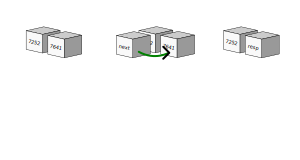
\includegraphics[width=\textwidth]{ortho-row1.pdf}
\end{frame}

\begin{frame}{Orthogonality issue}\Large
    \includegraphics[width=\textwidth]{ortho.pdf}
\end{frame}

\begin{frame}{Behavior definition: OSCORE}\Large
    \framesubtitle{Generalized from Observe behavior}

    \begin{itemize}
        \item Explicit request or not: Request needs sender and sequence number.
        \item Request nonce can only be used in one response.
        \item If order matters, responses are ordered by sequence number.
        \item If replaying matters, responses are subjected to the replay window.
        \item If follow-up requests were made, transiently tolerate erroneous responses.
    \end{itemize}
\end{frame}

\begin{frame}{Potential users}
\framesubtitle{Adapted from IETF113 slide set}

\begin{description}[oscore-capable-proxies]

\item[RFC7641] Observe notifications come in until further notice
\item[\sout{core-coap-sms}] Response-To-Uri-Host/-Port -- triangular requests
\item[\sout{core-coap-endpoint-id}] Observations across server address changes
\item[RFC8613] Explicit wording for Observe
\item[RFC9177] Responding with multiple blocks
\item[groupcomm-bis] Single request, different responses with different source addresses

    ← informative reference
\item[oscore-capable-proxies] to facilitate core-groupcomm-proxy's Multicast-Timeout

    ← TBD reference

\end{description}
\end{frame}

\begin{frame}{More in this document}\Large
     \begin{itemize}
         \item Define behavior of non-traditional responses in general
         \item Define new versatile non-traditional responses:
             \begin{itemize}\Large
                 \item Response-For
                 \item Leisure-For-Responses
                 \item Respond-To
             \end{itemize}
     \end{itemize}
\end{frame}

\begin{frame}{Next steps}\Large
    \begin{itemize}
        \item New options: illustrative or practical? (\href{https://github.com/core-wg/core-responses/issues/4}{\#4})
        \item Future in the WG?
    \end{itemize}
\end{frame}

\end{document}
